\subsection{KNN Results}\label{sec:res:knn}
We have evaluated the total 108 different KNN model configurations that can be achieved by assigning the different values available to each of the hyperparameters of the algorithm (k, distance metric, weighting method and voting policy).

We have trained and tested each of the KNN configurations on the 10 folds of each of the 2 datasets, and stored their achieved accuracy, time and F1 scores in 2 separate CSV files (one per dataset). In the following Subsections, we will discuss some metrics extracted from these results, and we will perform multiple statistical analyses in order to determine whether there are significant differences between the models or not.

\subsubsection{Hepatitis}
First of all, we summarize the obtained results in a pairplot matrix (Figure \ref{fig:hep:pairplot}). Each row and column of the matrix represents a hyperparameter, and the diagonal displays the accuracy histograms for each of the values of the corresponding hyperparameter. Meanwhile, the lower and upper triangles of the matrix display, respectively, the average accuracy and time heatmaps over the folds for each pairwise configurations of the 2 corresponding hyperparameters. With this kind of pairplot we get useful insight into the relationships betweem hyperparameters. We can see a clear trend towards better performance as the value of k goes up; however, this is a preliminary visualization and we cannot extract any real definitive conclusions.

Next, we filter out the top 10 performing models (based on average accuracy over the folds) and we perform a statistical analysis on them to try to find significant differences. After filtering the top 10 models, we apply a Friedman test on their accuracies over the 10 folds, with the null-hypothesis being that there is no significant difference between the models. From the Friedman test we obtain a p-value of \textbf{0.9997}, which overwhelmingly supports the null-hypothesis and indicates that \uline{there are not any statistically significant differences between the top 10 models}.

\begin{figure}[H]
    \centering
    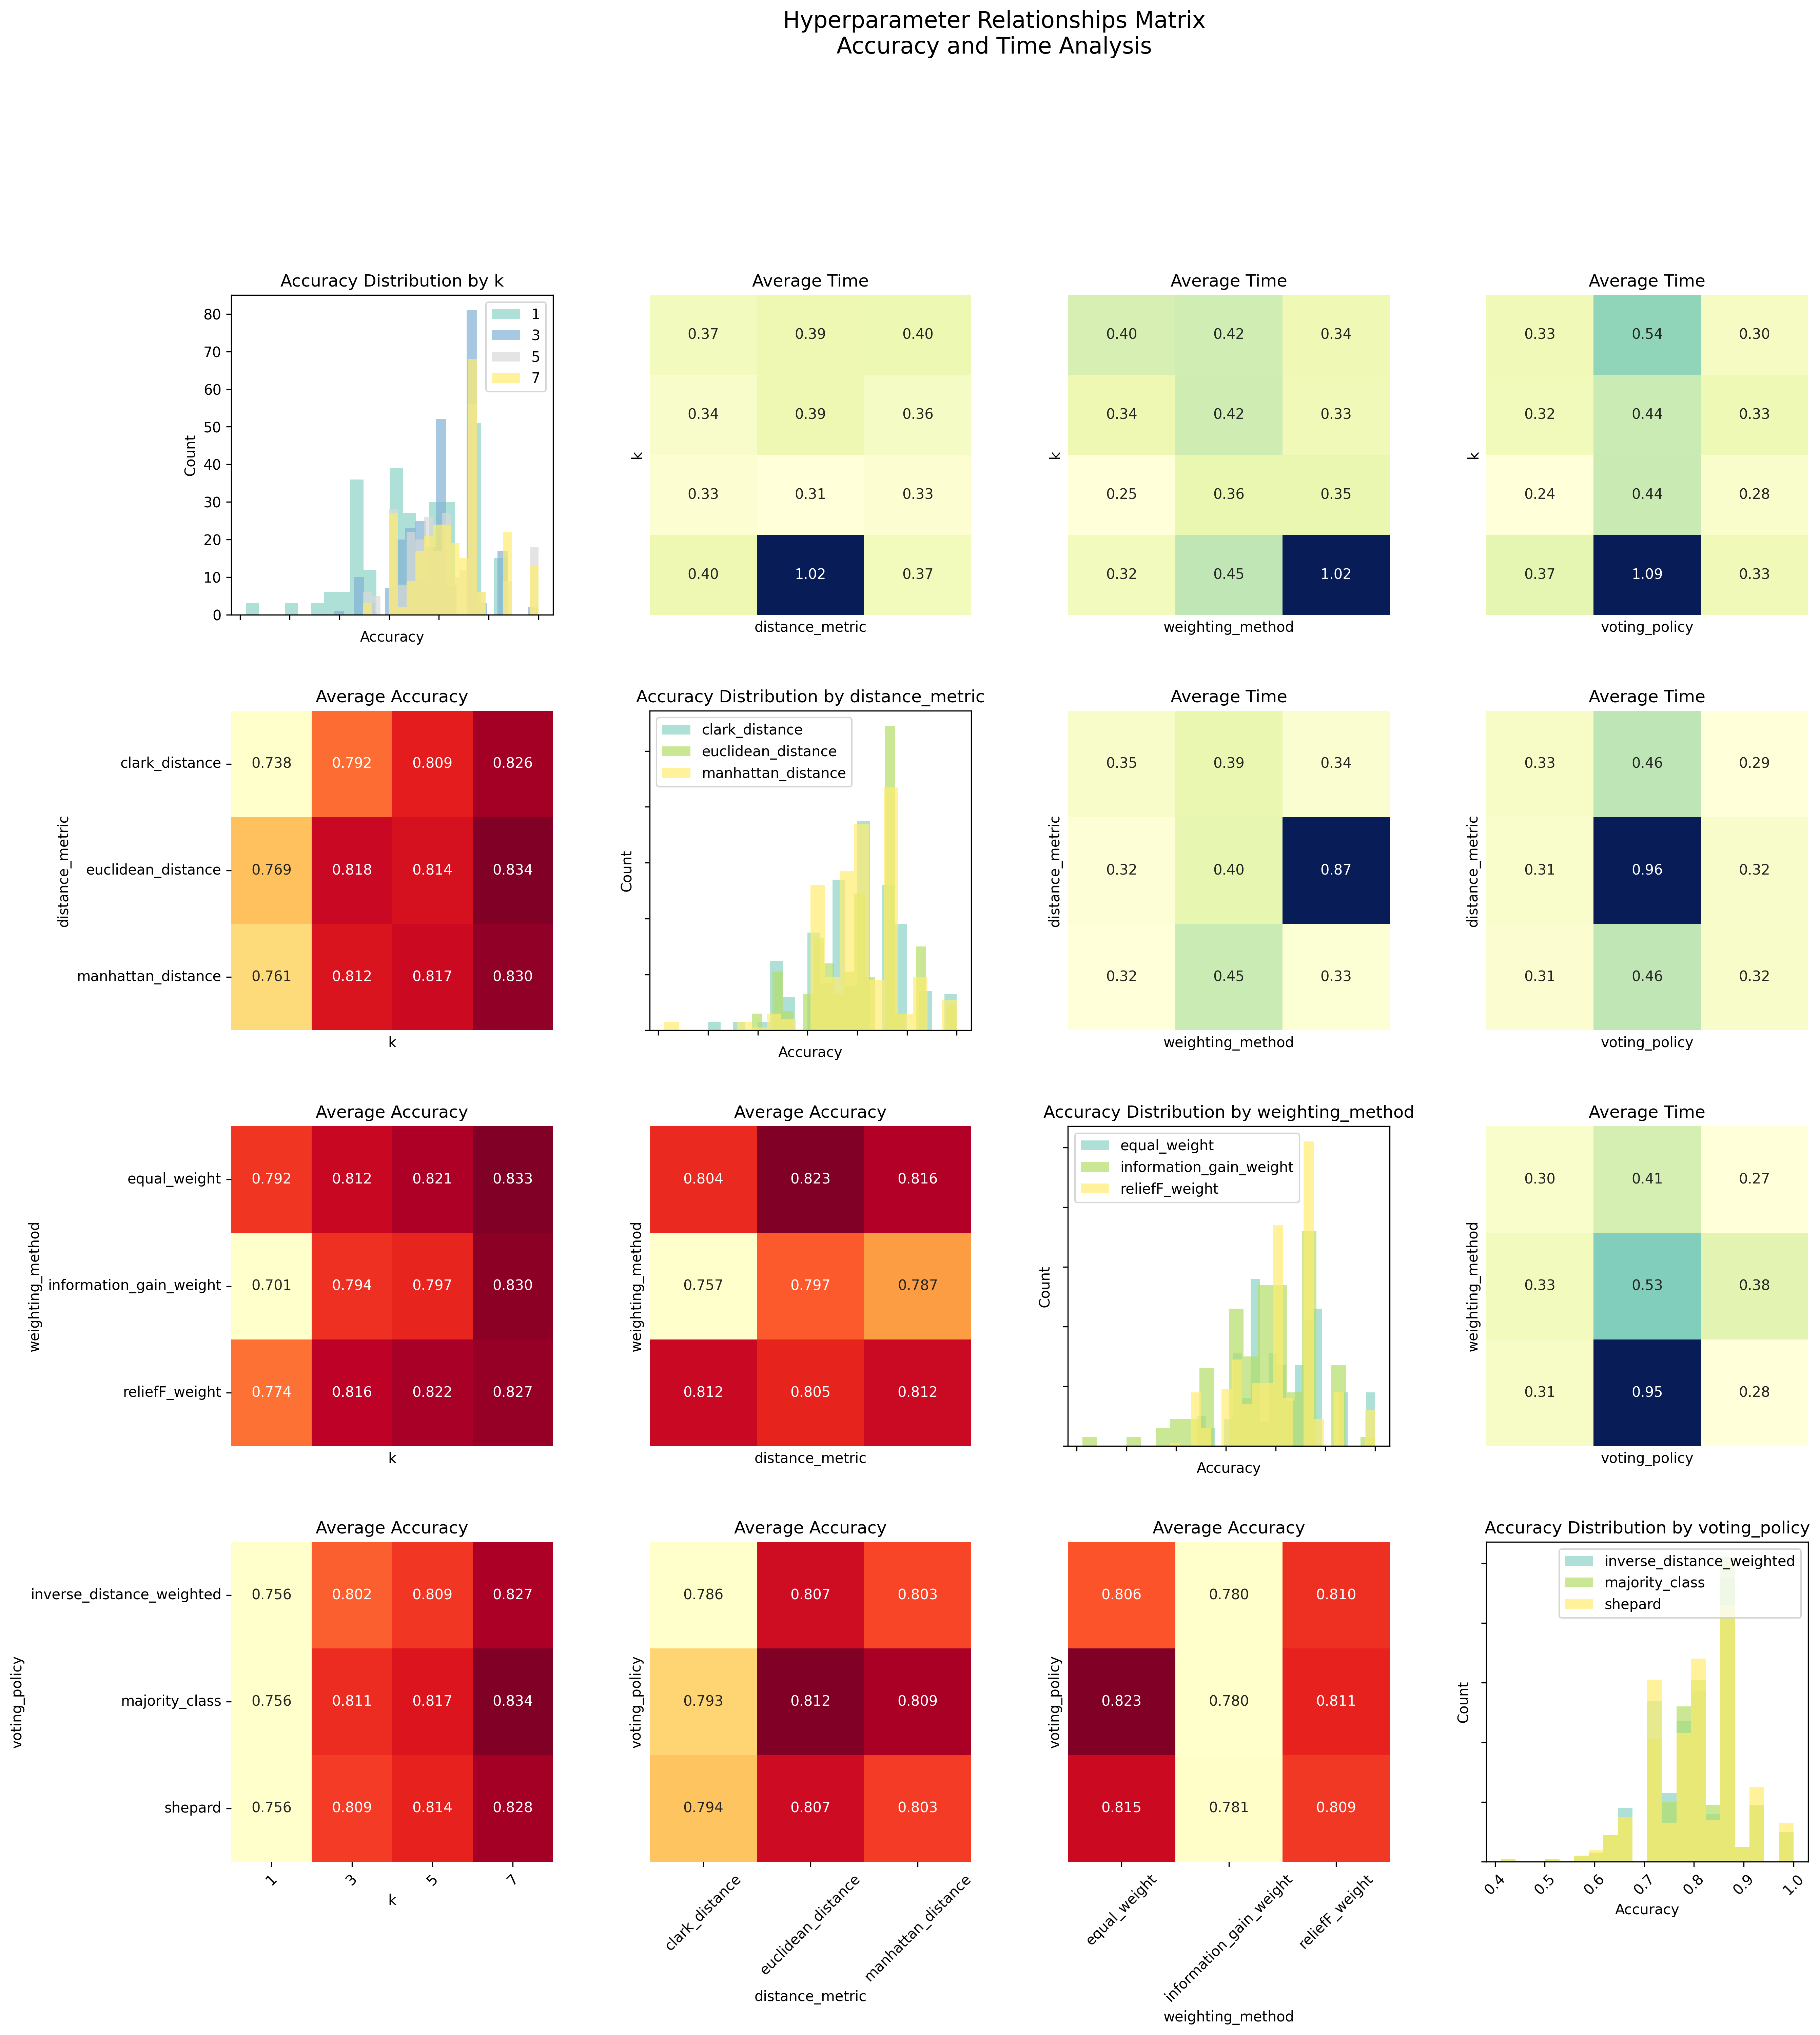
\includegraphics[width=\textwidth]{figures/knn/hepatitis/hyperparameter_pairplot_matrix.png}
    \caption{Hepatitis pairplot matrix summary}
    \label{fig:hep:pairplot}
\end{figure}
\FloatBarrier

Since we could not find a model that stands out over the rest with the standard statistical analysis over individual models, we now aim to at least find some indication as to which hyperparameter values are more prominent in succesful models. In order to do this, we performed 4 separate statistical tests by grouping the models according to their configuration of each of the hyperparameters. In other words, we applied a Friedman test to each of the hyperparameters to try to find significant differences between each of their possible values. The obtained p-values for each of the 4 Friedman tests can be seen in Table \ref{tab:knn:hep:hyperparam}.
\begin{table}[H]
    \centering
    \small
    \begin{tabular}{|c|c|c|c|}
        \hline
        \textbf{k} & \textbf{Distance metric} & \textbf{Weighting Method} & \textbf{Voting Policy} \\ \hline
        0.2071 & 0.2765 & 0.1211 & nan \\ \hline
    \end{tabular}
    \caption{Friedman test p-values per hyperparameter.}
    \label{tab:knn:hep:hyperparam}
\end{table}

If we set a level of significance of $ \alpha = 0.15 $ (which is already a relatively high value), we can only find significant differences between the different weighting methods. Note that the ``nan'' value in the test over the voting policy means that the ranks across the 4 different voting policies are identical, and therefore the Friedman test cannot be applied. This supports the null-hypothesis of not finding significant differences between the voting policies. We can see the results in Table \ref{tab:knn:hep:posthoc}.

Finally, we perform a post-hoc test on the weighting methods in order to further study the significant differences that we have found. In this case, the most appropriate post-hoc test to perform is the Bonferroni test with a control, since there is a clear ``standard'' choice of weighting method, which is Equal Weights, and we want to find if the other 2 weighting methods have any advantage over it.
\begin{table}[h!]
    \centering
    \small
    \begin{tabular}{|l|c|c|}
    \hline
                             & \textbf{p-value} & \textbf{Difference in accuracy (\%)} \\ \hline
    \textbf{Information Gain} & 0.2138           & -7.7961\%          \\ \hline
    \textbf{ReliefF}           & 0.1358           & -3.3461\%          \\ \hline
    \end{tabular}
    \caption{Results of the Bonferroni post-hoc test}
    \label{tab:knn:hep:posthoc}
\end{table}

Considering the calculated p-values, we can conclude that, with a significance level of $ \alpha = 0.15 $, \uline{we find statistically significant differences between the ReliefF weighting method and the control (Equal Weights), and we do not have strong enough evidence to support the same claim for the Information Gain method}. Looking at the average difference in accuracy percentage, we see that the ReliefF weighting method usually performs worse than Equal Weights on the Hepatitis dataset, and therefore we can conclude that it is siginificantly worse to utilize it instead of the standard Equal Weights when classifying samples of this dataset.

Before going to the next section, it is important to note that, since we did not find significant differences between the top performing KNN models, we can assume that all of the top models have statistically the same performance on the Hepatitis dataset. Hence, for simplicity's sake, we will take the one with the highest average accuracy rate (0.8519) in order to perform later tests of comparison between models, and between reduction methods. This model has a k value of 7, the Manhattan Distance, the Equal Weight method, and the Majority Class voting.

\subsubsection{Mushroom}
For the Mushroom dataset we will follow essentially the same steps as we did for the Hepatitis dataset, starting with visualizing the results in a pairplot matrix (Figure \ref{fig:mush:pairplot}). Interestingly, in this case we observe the opposite trend on the values of k as we did for the Hepatitis dataset, which indicates better perfomance of lower values of k this time. We can also see a tendency towards slightly better accuracy when using the Clark distance; however, we also observe extreme values of the computation time for said distance metric.

As we did before, we proceed with a Friedman test to try to find significant differences among the top performing models. This time we get a p-value of \textbf{nan}, which indicates that there is absolutely no difference in the ranks between the top 10 models. When observing the results, we find that all of the 10 models have an average accuracy of 1.0, which means that they all perfectly classify all of the test samples across the 10 folds of the Mushroom dataset. The only conclusion that we can take from this result is that \uline{the Mushroom dataset is not complex enough to show any difference in performance between these model configurations}.

\begin{figure}[H]
    \centering
    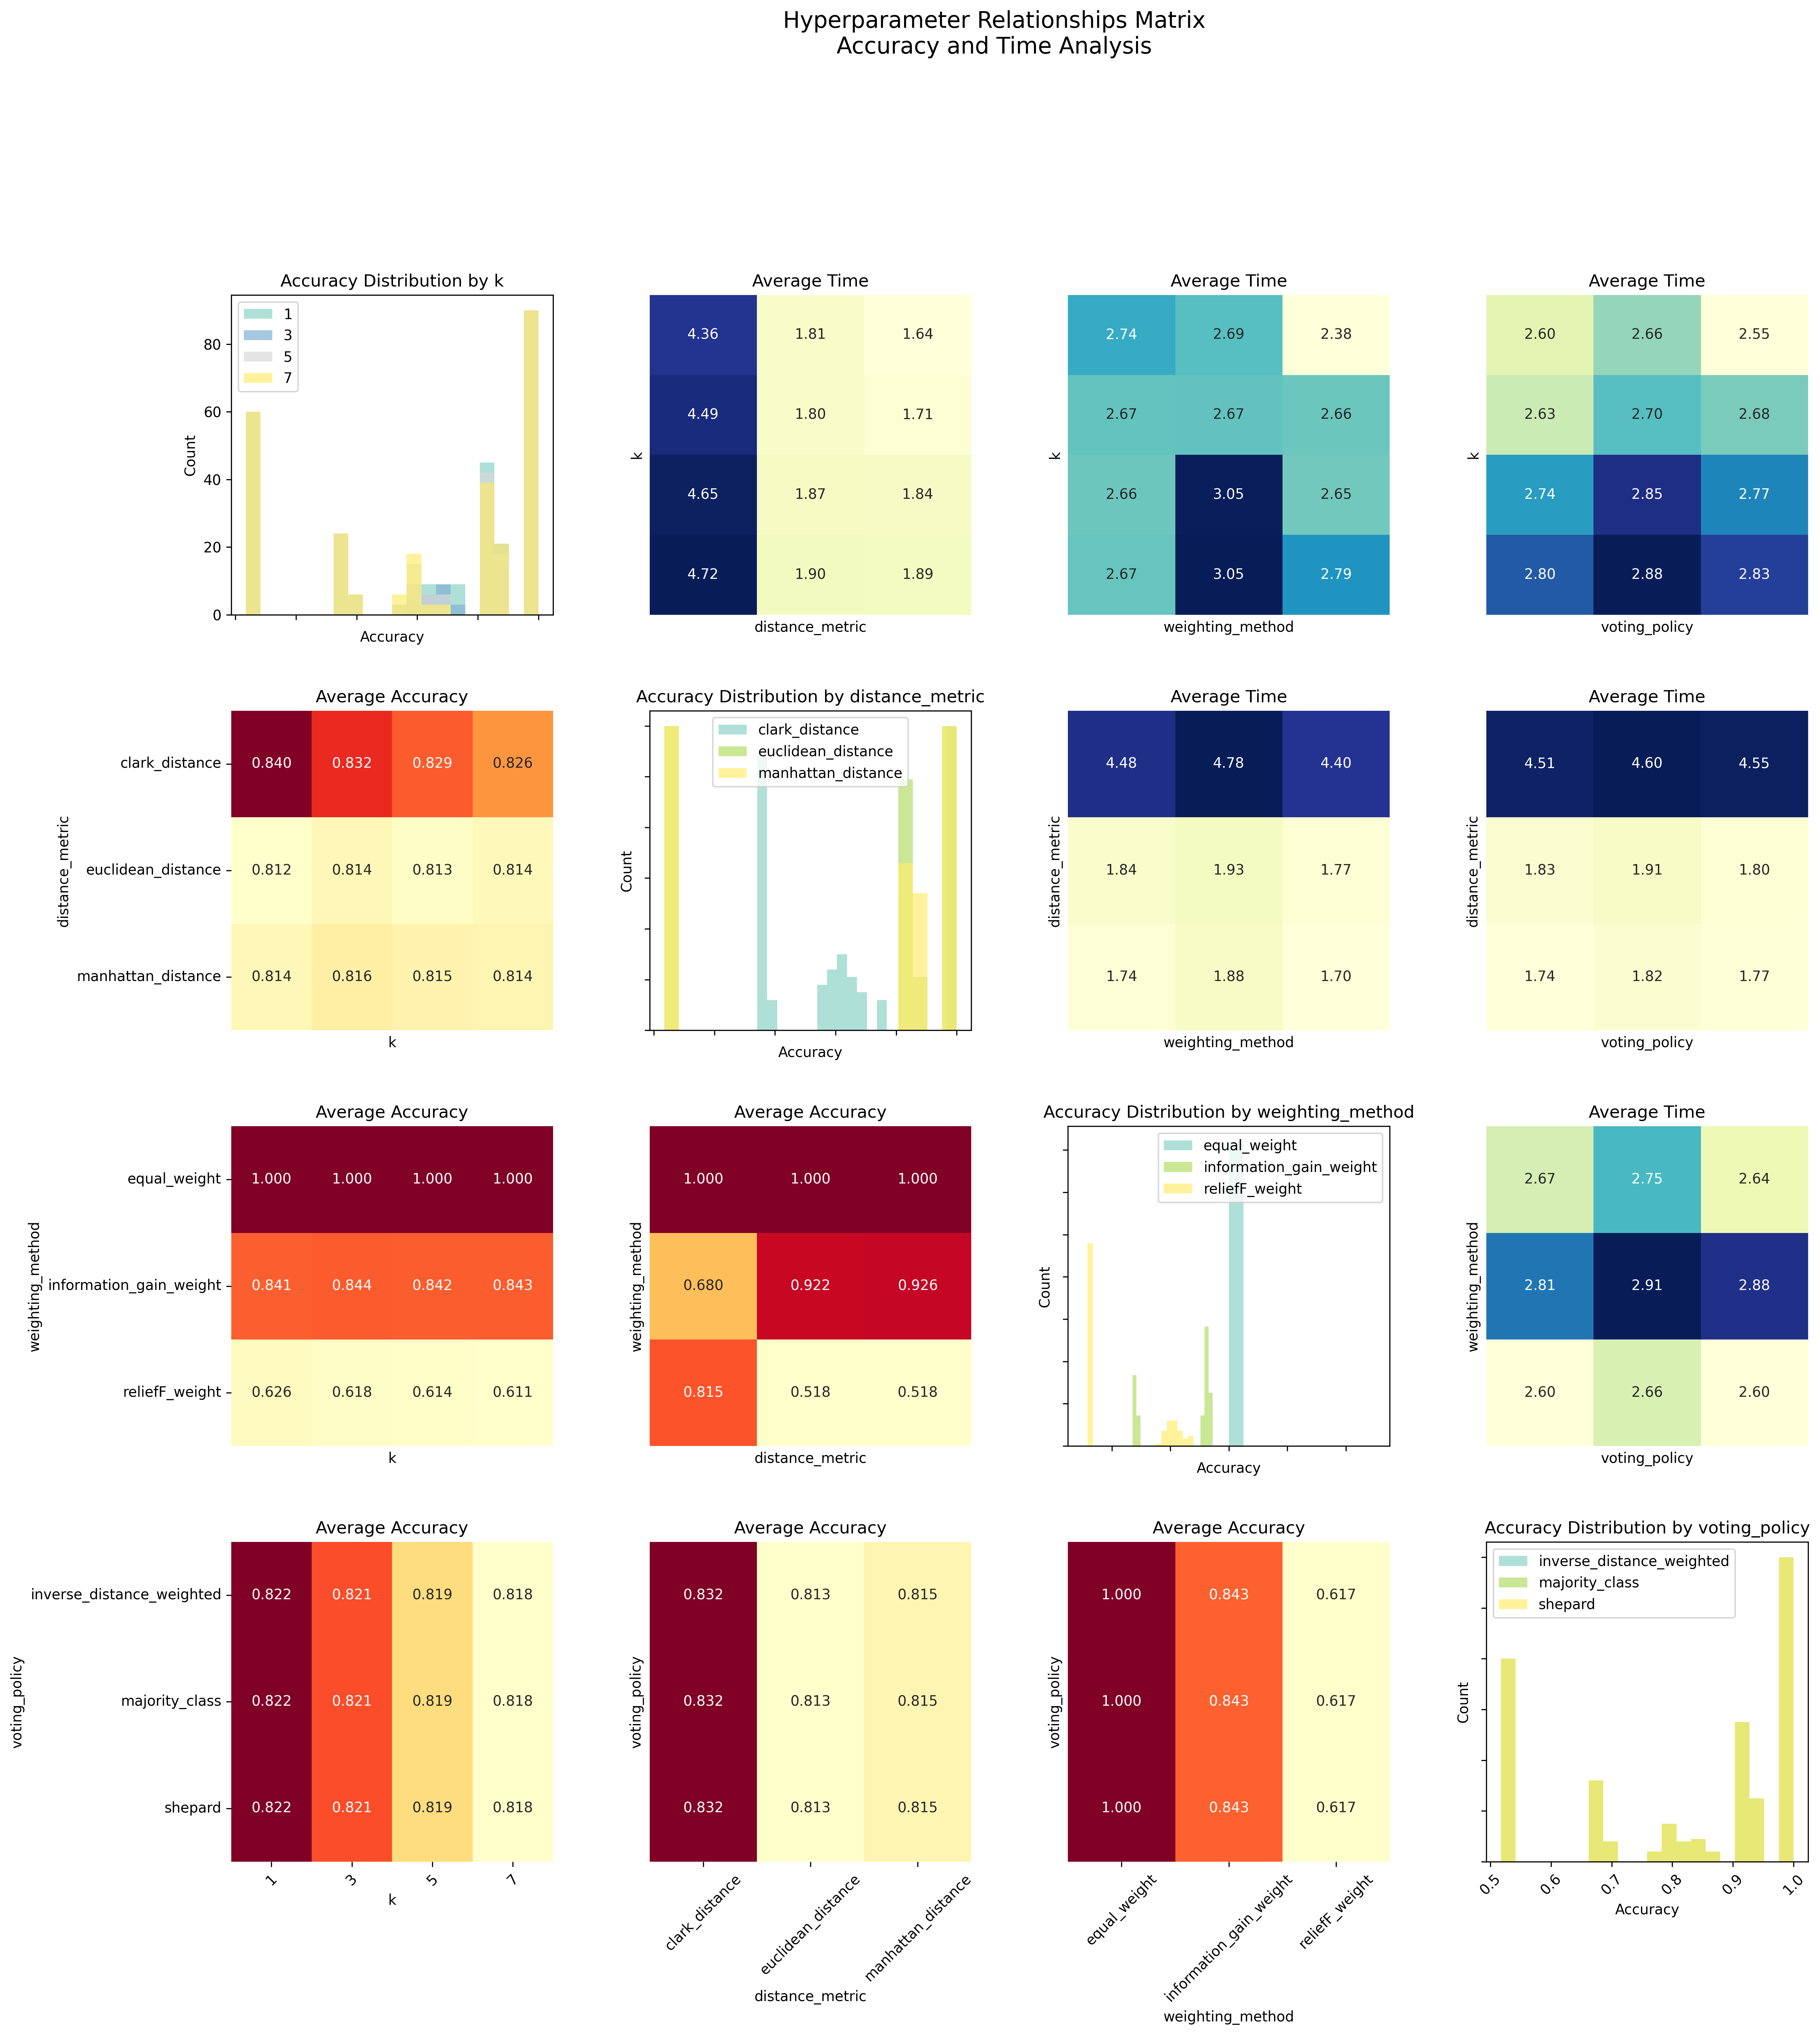
\includegraphics[width=\textwidth]{figures/knn/mushroom/hyperparameter_pairplot_matrix.png}
    \caption{Mushroom pairplot matrix summary}
    \label{fig:mush:pairplot}
\end{figure}
\FloatBarrier

Next, we perform a statistical test on the hyperparameters in order to find significant differences between their possible values. The results can be found in Table \ref{tab:knn:mush:hyperparam}.
\begin{table}[h]
    \centering
    \small
    \begin{tabular}{|c|c|c|c|}
        \hline
        \textbf{k} & \textbf{Distance metric} & \textbf{Weighting Method} & \textbf{Voting Policy} \\ \hline
        nan & nan & 0.0000 & nan \\ \hline
    \end{tabular}
    \caption{Friedman test p-values per hyperparameter.}
    \label{tab:knn:mush:hyperparam}
\end{table}

We see that the Friedman test cannot find any performance differences whatsoever between the different values of k, distance metric and voting policy. On the other hand, it is interesting to find that the p-value is \textbf{0.0000} for the weighting method, which essentially \textit{guarantees} (due to numerical approximation of the p-value) significant differences between the various weighting methods.

After applying the Bonferroni post-hoc test on the weighting methods, we get the results displayed on Table \ref{tab:knn:mush:posthoc}.
\begin{table}[h!]
    \centering
    \small
    \begin{tabular}{|l|c|c|}
    \hline
                             & \textbf{p-value} & \textbf{Difference in accuracy (\%)} \\ \hline
    \textbf{Information Gain} & 0.0039           & -8.0502\%          \\ \hline
    \textbf{ReliefF}           & 0.0039           & -48.2029\%          \\ \hline
    \end{tabular}
    \caption{Results of the Bonferroni post-hoc test}
    \label{tab:knn:mush:posthoc}
\end{table}

With these results, we can state that \uline{there is very strong evidence supporting that there is indeed significant differences between the Equal Weights method and the other 2}; since even with a significance level of $ \alpha = 0.01 $ (which is more stringent than the $ \alpha = 0.15 $ that we have for this test) we would reject the null-hypothesis. Looking at the average difference in accuracy percentage, we can see that both weighting methods show poorer average performance than the Equal Weights, and therefore it is detrimental to use them over the ``standard'' weighting method.

Similarly as with Hepatitis dataset, we could not find significant differences between the top performing models upon the Mushroom dataset. Therfore, for future comparisons we could utilize any of the top 10 models (all of them have accuracy rate of 1), so we choose one that seems to have the simplest configuration of hyperparameters: a k value of 1, the Euclidean Distance, the Equal Weight method, and Majority Class voting.